\documentclass[11pt,a4paper]{article}
\usepackage[utf8]{inputenc}
\usepackage[T1]{fontenc}
\renewcommand{\contentsname}{Sumário}\renewcommand{\figurename}{Figura}
\usepackage{amsmath,amssymb}
\usepackage{booktabs,array}
\usepackage{tikz}
\usetikzlibrary{positioning,calc}
\usepackage{listings}
\usepackage[margin=2.3cm]{geometry}
\usepackage[hidelinks]{hyperref}
\lstset{basicstyle=\ttfamily\footnotesize,frame=single,breaklines=true,columns=fullflexible,
  literate={á}{{\'a}}1 {é}{{\'e}}1 {í}{{\'i}}1 {ó}{{\'o}}1 {ã}{{\~a}}1 {ç}{{\c c}}1 {—}{{--}}1 {→}{{->}}1}
\newcommand{\at}{\mathit{at}}\newcommand{\lev}{\mathit{lev}}\newcommand{\clr}{\mathit{clr}}
\newcommand{\cov}{\mathit{cov}}\newcommand{\len}{\ell}\newcommand{\mv}{\mathit{move}}
\newcommand{\Tm}{\mathsf{T}}

\title{Manual de Resolução do Trabalho 01:\\ Mundo dos Blocos de Tamanho Variável via SAT Solver}
\author{Fundamentos de Inteligência Artificial --- Prof.\ Edjard Mota\\[6pt]
\textbf{Alunos:} André Cavalcanti, Tiago Gil de Brito, Ygor Gutierrz, Sofia Braga}
\date{2 de outubro de 2026}

\begin{document}
\maketitle
\tableofcontents

%====================================================================
\section{Introdução ao Problema}
O Mundo dos Blocos clássico tem blocos de tamanho 1 e uma única relação de apoio. Aqui os
blocos têm \emph{comprimentos diferentes} ($a,b$: 1uc; $c$: 2uc; $d$: 3uc), ocupam
posições horizontais livres sobre uma mesa de 6 slots, podem deixar espaços vazios, deslizar
lateralmente e ficar em \emph{ponte} sobre dois apoios. Um bloco só é estável se tiver
apoio suficiente. O objetivo é, dado um estado inicial $S_0$ e um estado-meta, obter um plano
(sequência de ações \texttt{move}) e provar sua otimalidade com um SAT solver.

O trabalho cobre três cenários (Situações 1, 2 e 3 do enunciado). O fluxo seguido foi:
(i) modelagem em lógica de primeira ordem (LPO); (ii) resolução \emph{manual} dos cenários;
(iii) codificação proposicional (CNF); (iv) execução do SAT solver e interpretação; (v) comparação
com os planos manuais e com um planejador BFS independente (oráculo).

%====================================================================
\section{Descrição Formal do Mundo dos Blocos de Tamanho Variado}
\subsection{Domínio}
$B=\{a,b,c,d\}$; $L=B\cup\{\Tm\}$ (locais de apoio, $\Tm$ = mesa); $\len(a)=\len(b)=1$,
$\len(c)=2$, $\len(d)=3$. O eixo tem os \emph{pontos} $X=\{0,\dots,6\}$ e os \emph{slots}
$s_i=[i,i+1]$, $i\in\{0,\dots,5\}$ (6 slots, não 7). Um bloco que começa no ponto $p$ cobre os slots
$\{p,\dots,p+\len(b)-1\}$; as posições válidas são $p\in\{0,\dots,6-\len(b)\}$. Os níveis são
$0$ (mesa) a $3$.

\subsection{Representação em LPO}
Usamos o cálculo de situações: $s$ é uma situação e $do(\alpha,s)$ a situação após a ação $\alpha$.

\paragraph{Fluentes primitivos.}
$\at(b,p,s)$: $b$ começa no ponto $p$; $\lev(b,l,s)$: $b$ está no nível $l$.

\paragraph{Relações derivadas} (definidas por equivalência, nunca armazenadas):
\begin{align*}
\cov(b,k,l,s) &\leftrightarrow \exists p.\ \at(b,p,s)\wedge\lev(b,l,s)\wedge p\le k<p+\len(b)\\
\mathit{free}(k,l,s) &\leftrightarrow \neg\exists x.\ \cov(x,k,l,s)\\
\mathit{on}(b,y,s) &\leftrightarrow \exists k.\ \cov(b,k,l,s)\wedge\cov(y,k,l-1,s)\quad(\text{e }\mathit{on}(b,\Tm,s)\leftrightarrow\lev(b,0,s))\\
\clr(b,s) &\leftrightarrow \neg\exists x,k.\ \cov(b,k,l,s)\wedge\lev(b,l,s)\wedge\cov(x,k,l+1,s)\\
\mathit{stable}(b,p,l,s) &\leftrightarrow l=0\ \vee\ \#\{k\in[p,p+\len(b)-1]:\exists y\neq b.\ \cov(y,k,l-1,s)\}\ \ge\ \lceil\len(b)/2\rceil
\end{align*}
Como $\mathit{on}$ é derivada, um bloco pode ter vários apoios (ponte): $\mathit{on}(d,a,s)\wedge\mathit{on}(d,b,s)$.

\paragraph{Ação.} $\mv(b,y,p)$: ``mover $b$ para cima de $y\in(B\setminus\{b\})\cup\{\Tm\}$, começando no ponto $p$''.
Seja $l_y(s)=0$ se $y=\Tm$ e $l_y(s)=l'+1$ se $\lev(y,l',s)$ (nível de destino).
\begin{align*}
Poss(\mv(b,y,p),s)\leftrightarrow\ & \clr(b,s)\ \wedge\ \neg(\at(b,p,s)\wedge\lev(b,l_y(s),s))\\
&\wedge\ (y\in B\to\exists k\in[p,p+\len(b)-1].\ \cov(y,k,l_y(s)-1,s))\\
&\wedge\ \forall k\in[p,p+\len(b)-1].\ \forall x\neq b.\ \neg\cov(x,k,l_y(s),s)\\
&\wedge\ \mathit{stable}(b,p,l_y(s),s)\ \wedge\ l_y(s)\le 3
\end{align*}
Axiomas de estado sucessor, para $\alpha=\mv(b,y,p)$ e $l=l_y(s)$:
\begin{align*}
\at(x,q,do(\alpha,s))&\leftrightarrow (x=b\wedge q=p)\ \vee\ (\at(x,q,s)\wedge x\neq b)\\
\lev(x,m,do(\alpha,s))&\leftrightarrow (x=b\wedge m=l)\ \vee\ (\lev(x,m,s)\wedge x\neq b)
\end{align*}

\subsection{Elementos novos e ações associadas (adds/deletes)}
\begin{center}\small
\begin{tabular}{@{}p{3.0cm}p{2.3cm}p{3.5cm}p{4.0cm}@{}}\toprule
Elemento & Tipo & Add & Delete\\\midrule
$\len(b)$, $B$, $X$ & termos/constantes & --- & --- (rígidos)\\
$\at(b,p)$ & fluente & $\at(b,p)$ & $\at(b,p_0)$ antigo\\
$\lev(b,l)$ & fluente & $\lev(b,l_y+1)$ (ou $0$) & $\lev(b,l_0)$ antigo\\
$\clr(y)$ & derivado & --- & deixa de valer se $b$ passa a cobrir $y$\\
$\clr(z)$, $z$ antigo apoio & derivado & vale se nada mais o cobre & ---\\
$\mathit{on}(b,y)$ & derivado & novos apoios sob $[p,p+\len(b))$ & apoios antigos\\
$\mathit{stable}$ & pré-condição & --- & ---\\
$\mathit{free}(k,l)$ & derivado & células deixadas por $b$ & células ocupadas por $b$\\\bottomrule
\end{tabular}\end{center}
Só $\at$ e $\lev$ são alterados pela ação; tudo o mais é recalculado, o que elimina os axiomas de frame para $\clr$ e $\mathit{on}$.
\emph{Correção em relação ao esboço do manual:} não se exige $\clr(y)$ para o destino $y$; basta que os slots-alvo estejam livres. Exigir $\clr(y)$ tornaria inalcançáveis os estados com dois blocos sobre $c$ (por exemplo $S_7$).

\subsection{Ordem parcial ($A\xrightarrow{P}B$)}
Um plano é uma ordem parcial de ações com \emph{ligações causais} $A\xrightarrow{P}B$: $A$ produz $P$ e $B$ consome $P$, sem
que nenhuma ação intermediária desfaça $P$. Em nossa representação, $P$ é uma \emph{célula} $(\text{slot},\text{nível})$ ou a posição de um bloco.
Para cada ação $\alpha=\mv(b,y,p)$ definimos:
\begin{align*}
W(\alpha)&=\{\mathit{pos}(b)\}\cup\mathit{celulas\_antigas}(b)\cup\mathit{celulas\_novas}(b)\\
R(\alpha)&=\{\mathit{pos}(y)\}\cup\mathit{celulas\_acima\_antigas}(b)\cup\mathit{apoio\_novo}(b)\cup\mathit{celulas\_novas}(b)
\end{align*}
$\alpha_i\prec\alpha_j$ se $i<j$ e $W_i\cap R_j\neq\emptyset$ (ligação causal $\alpha_i\xrightarrow{P}\alpha_j$),
$W_i\cap W_j\neq\emptyset$ ou $R_i\cap W_j\neq\emptyset$ (proteção). Ações sem relação são \emph{independentes}: qualquer ordem
é válida. O fecho transitivo é reduzido (diagrama de Hasse) em \texttt{interpretar.py}, que também \emph{verifica} que toda linearização é executável.

\subsection{Resolução manual}
Notação: $x@p/l$ = bloco $x$ no ponto $p$, nível $l$. Em todo passo foram verificados: topo livre, slots-alvo livres no nível de destino e apoio $\ge\lceil\len/2\rceil$.
Os cenários estão desenhados abaixo.
\begin{figure}[h]\centering\begin{minipage}[b]{0.31\textwidth}\centering
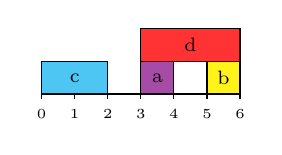
\begin{tikzpicture}[x=0.42cm,y=0.42cm,font=\scriptsize]
\draw[fill=cyan!70] (0,0) rectangle (2,1);\node at (1.0,0.5) {c};
\draw[fill=violet!70] (3,0) rectangle (4,1);\node at (3.5,0.5) {a};
\draw[fill=yellow!90] (5,0) rectangle (6,1);\node at (5.5,0.5) {b};
\draw[fill=red!80] (3,1) rectangle (6,2);\node at (4.5,1.5) {d};
\draw[thick] (0,0) -- (6,0);
\draw (0,0) -- (0,-0.15) node[below,font=\tiny] {0};
\draw (1,0) -- (1,-0.15) node[below,font=\tiny] {1};
\draw (2,0) -- (2,-0.15) node[below,font=\tiny] {2};
\draw (3,0) -- (3,-0.15) node[below,font=\tiny] {3};
\draw (4,0) -- (4,-0.15) node[below,font=\tiny] {4};
\draw (5,0) -- (5,-0.15) node[below,font=\tiny] {5};
\draw (6,0) -- (6,-0.15) node[below,font=\tiny] {6};
\end{tikzpicture}\\[2pt] $S_0$\end{minipage}\hfill
\begin{minipage}[b]{0.31\textwidth}\centering
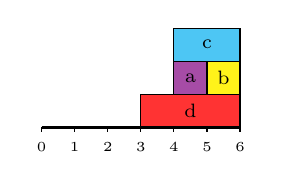
\begin{tikzpicture}[x=0.42cm,y=0.42cm,font=\scriptsize]
\draw[fill=red!80] (3,0) rectangle (6,1);\node at (4.5,0.5) {d};
\draw[fill=violet!70] (4,1) rectangle (5,2);\node at (4.5,1.5) {a};
\draw[fill=yellow!90] (5,1) rectangle (6,2);\node at (5.5,1.5) {b};
\draw[fill=cyan!70] (4,2) rectangle (6,3);\node at (5.0,2.5) {c};
\draw[thick] (0,0) -- (6,0);
\draw (0,0) -- (0,-0.15) node[below,font=\tiny] {0};
\draw (1,0) -- (1,-0.15) node[below,font=\tiny] {1};
\draw (2,0) -- (2,-0.15) node[below,font=\tiny] {2};
\draw (3,0) -- (3,-0.15) node[below,font=\tiny] {3};
\draw (4,0) -- (4,-0.15) node[below,font=\tiny] {4};
\draw (5,0) -- (5,-0.15) node[below,font=\tiny] {5};
\draw (6,0) -- (6,-0.15) node[below,font=\tiny] {6};
\end{tikzpicture}\\[2pt] $S_{f1}$\end{minipage}\hfill
\begin{minipage}[b]{0.31\textwidth}\centering
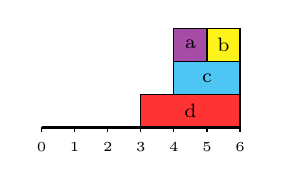
\begin{tikzpicture}[x=0.42cm,y=0.42cm,font=\scriptsize]
\draw[fill=red!80] (3,0) rectangle (6,1);\node at (4.5,0.5) {d};
\draw[fill=cyan!70] (4,1) rectangle (6,2);\node at (5.0,1.5) {c};
\draw[fill=violet!70] (4,2) rectangle (5,3);\node at (4.5,2.5) {a};
\draw[fill=yellow!90] (5,2) rectangle (6,3);\node at (5.5,2.5) {b};
\draw[thick] (0,0) -- (6,0);
\draw (0,0) -- (0,-0.15) node[below,font=\tiny] {0};
\draw (1,0) -- (1,-0.15) node[below,font=\tiny] {1};
\draw (2,0) -- (2,-0.15) node[below,font=\tiny] {2};
\draw (3,0) -- (3,-0.15) node[below,font=\tiny] {3};
\draw (4,0) -- (4,-0.15) node[below,font=\tiny] {4};
\draw (5,0) -- (5,-0.15) node[below,font=\tiny] {5};
\draw (6,0) -- (6,-0.15) node[below,font=\tiny] {6};
\end{tikzpicture}\\[2pt] $S_{f2}$\end{minipage}\\[8pt]
\begin{minipage}[b]{0.31\textwidth}\centering
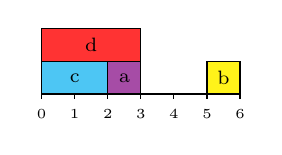
\begin{tikzpicture}[x=0.42cm,y=0.42cm,font=\scriptsize]
\draw[fill=cyan!70] (0,0) rectangle (2,1);\node at (1.0,0.5) {c};
\draw[fill=violet!70] (2,0) rectangle (3,1);\node at (2.5,0.5) {a};
\draw[fill=yellow!90] (5,0) rectangle (6,1);\node at (5.5,0.5) {b};
\draw[fill=red!80] (0,1) rectangle (3,2);\node at (1.5,1.5) {d};
\draw[thick] (0,0) -- (6,0);
\draw (0,0) -- (0,-0.15) node[below,font=\tiny] {0};
\draw (1,0) -- (1,-0.15) node[below,font=\tiny] {1};
\draw (2,0) -- (2,-0.15) node[below,font=\tiny] {2};
\draw (3,0) -- (3,-0.15) node[below,font=\tiny] {3};
\draw (4,0) -- (4,-0.15) node[below,font=\tiny] {4};
\draw (5,0) -- (5,-0.15) node[below,font=\tiny] {5};
\draw (6,0) -- (6,-0.15) node[below,font=\tiny] {6};
\end{tikzpicture}\\[2pt] $S_{f3}$\end{minipage}\hfill
\begin{minipage}[b]{0.31\textwidth}\centering
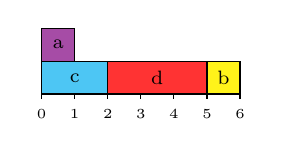
\begin{tikzpicture}[x=0.42cm,y=0.42cm,font=\scriptsize]
\draw[fill=cyan!70] (0,0) rectangle (2,1);\node at (1.0,0.5) {c};
\draw[fill=red!80] (2,0) rectangle (5,1);\node at (3.5,0.5) {d};
\draw[fill=yellow!90] (5,0) rectangle (6,1);\node at (5.5,0.5) {b};
\draw[fill=violet!70] (0,1) rectangle (1,2);\node at (0.5,1.5) {a};
\draw[thick] (0,0) -- (6,0);
\draw (0,0) -- (0,-0.15) node[below,font=\tiny] {0};
\draw (1,0) -- (1,-0.15) node[below,font=\tiny] {1};
\draw (2,0) -- (2,-0.15) node[below,font=\tiny] {2};
\draw (3,0) -- (3,-0.15) node[below,font=\tiny] {3};
\draw (4,0) -- (4,-0.15) node[below,font=\tiny] {4};
\draw (5,0) -- (5,-0.15) node[below,font=\tiny] {5};
\draw (6,0) -- (6,-0.15) node[below,font=\tiny] {6};
\end{tikzpicture}\\[2pt] $S_{f4}$\end{minipage}\hfill\caption{Situação 1: $S_0$ e $S_{f1}$--$S_{f4}$.}\end{figure}
\begin{figure}[h]\centering\begin{minipage}[b]{0.31\textwidth}\centering
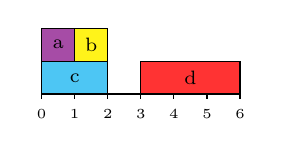
\begin{tikzpicture}[x=0.42cm,y=0.42cm,font=\scriptsize]
\draw[fill=cyan!70] (0,0) rectangle (2,1);\node at (1.0,0.5) {c};
\draw[fill=red!80] (3,0) rectangle (6,1);\node at (4.5,0.5) {d};
\draw[fill=violet!70] (0,1) rectangle (1,2);\node at (0.5,1.5) {a};
\draw[fill=yellow!90] (1,1) rectangle (2,2);\node at (1.5,1.5) {b};
\draw[thick] (0,0) -- (6,0);
\draw (0,0) -- (0,-0.15) node[below,font=\tiny] {0};
\draw (1,0) -- (1,-0.15) node[below,font=\tiny] {1};
\draw (2,0) -- (2,-0.15) node[below,font=\tiny] {2};
\draw (3,0) -- (3,-0.15) node[below,font=\tiny] {3};
\draw (4,0) -- (4,-0.15) node[below,font=\tiny] {4};
\draw (5,0) -- (5,-0.15) node[below,font=\tiny] {5};
\draw (6,0) -- (6,-0.15) node[below,font=\tiny] {6};
\end{tikzpicture}\\[2pt] $S_0$\end{minipage}\hfill
\begin{minipage}[b]{0.31\textwidth}\centering
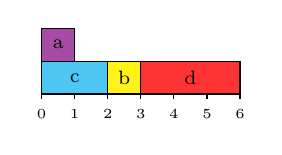
\begin{tikzpicture}[x=0.42cm,y=0.42cm,font=\scriptsize]
\draw[fill=cyan!70] (0,0) rectangle (2,1);\node at (1.0,0.5) {c};
\draw[fill=yellow!90] (2,0) rectangle (3,1);\node at (2.5,0.5) {b};
\draw[fill=red!80] (3,0) rectangle (6,1);\node at (4.5,0.5) {d};
\draw[fill=violet!70] (0,1) rectangle (1,2);\node at (0.5,1.5) {a};
\draw[thick] (0,0) -- (6,0);
\draw (0,0) -- (0,-0.15) node[below,font=\tiny] {0};
\draw (1,0) -- (1,-0.15) node[below,font=\tiny] {1};
\draw (2,0) -- (2,-0.15) node[below,font=\tiny] {2};
\draw (3,0) -- (3,-0.15) node[below,font=\tiny] {3};
\draw (4,0) -- (4,-0.15) node[below,font=\tiny] {4};
\draw (5,0) -- (5,-0.15) node[below,font=\tiny] {5};
\draw (6,0) -- (6,-0.15) node[below,font=\tiny] {6};
\end{tikzpicture}\\[2pt] $S_{1}$\end{minipage}\hfill
\begin{minipage}[b]{0.31\textwidth}\centering
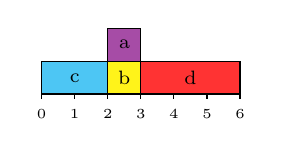
\begin{tikzpicture}[x=0.42cm,y=0.42cm,font=\scriptsize]
\draw[fill=cyan!70] (0,0) rectangle (2,1);\node at (1.0,0.5) {c};
\draw[fill=yellow!90] (2,0) rectangle (3,1);\node at (2.5,0.5) {b};
\draw[fill=red!80] (3,0) rectangle (6,1);\node at (4.5,0.5) {d};
\draw[fill=violet!70] (2,1) rectangle (3,2);\node at (2.5,1.5) {a};
\draw[thick] (0,0) -- (6,0);
\draw (0,0) -- (0,-0.15) node[below,font=\tiny] {0};
\draw (1,0) -- (1,-0.15) node[below,font=\tiny] {1};
\draw (2,0) -- (2,-0.15) node[below,font=\tiny] {2};
\draw (3,0) -- (3,-0.15) node[below,font=\tiny] {3};
\draw (4,0) -- (4,-0.15) node[below,font=\tiny] {4};
\draw (5,0) -- (5,-0.15) node[below,font=\tiny] {5};
\draw (6,0) -- (6,-0.15) node[below,font=\tiny] {6};
\end{tikzpicture}\\[2pt] $S_{2}$\end{minipage}\\[8pt]
\begin{minipage}[b]{0.31\textwidth}\centering
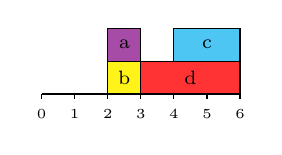
\begin{tikzpicture}[x=0.42cm,y=0.42cm,font=\scriptsize]
\draw[fill=yellow!90] (2,0) rectangle (3,1);\node at (2.5,0.5) {b};
\draw[fill=red!80] (3,0) rectangle (6,1);\node at (4.5,0.5) {d};
\draw[fill=violet!70] (2,1) rectangle (3,2);\node at (2.5,1.5) {a};
\draw[fill=cyan!70] (4,1) rectangle (6,2);\node at (5.0,1.5) {c};
\draw[thick] (0,0) -- (6,0);
\draw (0,0) -- (0,-0.15) node[below,font=\tiny] {0};
\draw (1,0) -- (1,-0.15) node[below,font=\tiny] {1};
\draw (2,0) -- (2,-0.15) node[below,font=\tiny] {2};
\draw (3,0) -- (3,-0.15) node[below,font=\tiny] {3};
\draw (4,0) -- (4,-0.15) node[below,font=\tiny] {4};
\draw (5,0) -- (5,-0.15) node[below,font=\tiny] {5};
\draw (6,0) -- (6,-0.15) node[below,font=\tiny] {6};
\end{tikzpicture}\\[2pt] $S_{3}$\end{minipage}\hfill
\begin{minipage}[b]{0.31\textwidth}\centering
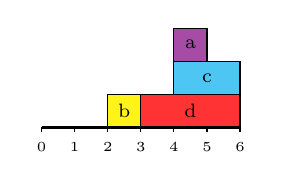
\begin{tikzpicture}[x=0.42cm,y=0.42cm,font=\scriptsize]
\draw[fill=yellow!90] (2,0) rectangle (3,1);\node at (2.5,0.5) {b};
\draw[fill=red!80] (3,0) rectangle (6,1);\node at (4.5,0.5) {d};
\draw[fill=cyan!70] (4,1) rectangle (6,2);\node at (5.0,1.5) {c};
\draw[fill=violet!70] (4,2) rectangle (5,3);\node at (4.5,2.5) {a};
\draw[thick] (0,0) -- (6,0);
\draw (0,0) -- (0,-0.15) node[below,font=\tiny] {0};
\draw (1,0) -- (1,-0.15) node[below,font=\tiny] {1};
\draw (2,0) -- (2,-0.15) node[below,font=\tiny] {2};
\draw (3,0) -- (3,-0.15) node[below,font=\tiny] {3};
\draw (4,0) -- (4,-0.15) node[below,font=\tiny] {4};
\draw (5,0) -- (5,-0.15) node[below,font=\tiny] {5};
\draw (6,0) -- (6,-0.15) node[below,font=\tiny] {6};
\end{tikzpicture}\\[2pt] $S_{4}$\end{minipage}\hfill
\begin{minipage}[b]{0.31\textwidth}\centering
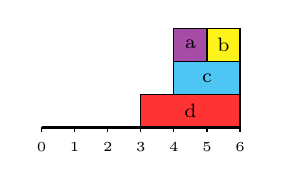
\begin{tikzpicture}[x=0.42cm,y=0.42cm,font=\scriptsize]
\draw[fill=red!80] (3,0) rectangle (6,1);\node at (4.5,0.5) {d};
\draw[fill=cyan!70] (4,1) rectangle (6,2);\node at (5.0,1.5) {c};
\draw[fill=violet!70] (4,2) rectangle (5,3);\node at (4.5,2.5) {a};
\draw[fill=yellow!90] (5,2) rectangle (6,3);\node at (5.5,2.5) {b};
\draw[thick] (0,0) -- (6,0);
\draw (0,0) -- (0,-0.15) node[below,font=\tiny] {0};
\draw (1,0) -- (1,-0.15) node[below,font=\tiny] {1};
\draw (2,0) -- (2,-0.15) node[below,font=\tiny] {2};
\draw (3,0) -- (3,-0.15) node[below,font=\tiny] {3};
\draw (4,0) -- (4,-0.15) node[below,font=\tiny] {4};
\draw (5,0) -- (5,-0.15) node[below,font=\tiny] {5};
\draw (6,0) -- (6,-0.15) node[below,font=\tiny] {6};
\end{tikzpicture}\\[2pt] $S_{5}$\end{minipage}\\[8pt]\caption{Situação 2: $S_0$ a $S_5$.}\end{figure}
\begin{figure}[h]\centering\begin{minipage}[b]{0.31\textwidth}\centering
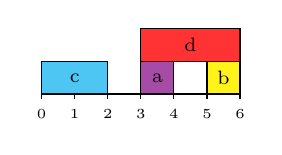
\begin{tikzpicture}[x=0.42cm,y=0.42cm,font=\scriptsize]
\draw[fill=cyan!70] (0,0) rectangle (2,1);\node at (1.0,0.5) {c};
\draw[fill=violet!70] (3,0) rectangle (4,1);\node at (3.5,0.5) {a};
\draw[fill=yellow!90] (5,0) rectangle (6,1);\node at (5.5,0.5) {b};
\draw[fill=red!80] (3,1) rectangle (6,2);\node at (4.5,1.5) {d};
\draw[thick] (0,0) -- (6,0);
\draw (0,0) -- (0,-0.15) node[below,font=\tiny] {0};
\draw (1,0) -- (1,-0.15) node[below,font=\tiny] {1};
\draw (2,0) -- (2,-0.15) node[below,font=\tiny] {2};
\draw (3,0) -- (3,-0.15) node[below,font=\tiny] {3};
\draw (4,0) -- (4,-0.15) node[below,font=\tiny] {4};
\draw (5,0) -- (5,-0.15) node[below,font=\tiny] {5};
\draw (6,0) -- (6,-0.15) node[below,font=\tiny] {6};
\end{tikzpicture}\\[2pt] $S_0$\end{minipage}\hfill
\begin{minipage}[b]{0.31\textwidth}\centering
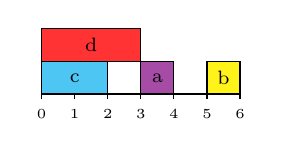
\begin{tikzpicture}[x=0.42cm,y=0.42cm,font=\scriptsize]
\draw[fill=cyan!70] (0,0) rectangle (2,1);\node at (1.0,0.5) {c};
\draw[fill=red!80] (0,1) rectangle (3,2);\node at (1.5,1.5) {d};
\draw[fill=violet!70] (3,0) rectangle (4,1);\node at (3.5,0.5) {a};
\draw[fill=yellow!90] (5,0) rectangle (6,1);\node at (5.5,0.5) {b};
\draw[thick] (0,0) -- (6,0);
\draw (0,0) -- (0,-0.15) node[below,font=\tiny] {0};
\draw (1,0) -- (1,-0.15) node[below,font=\tiny] {1};
\draw (2,0) -- (2,-0.15) node[below,font=\tiny] {2};
\draw (3,0) -- (3,-0.15) node[below,font=\tiny] {3};
\draw (4,0) -- (4,-0.15) node[below,font=\tiny] {4};
\draw (5,0) -- (5,-0.15) node[below,font=\tiny] {5};
\draw (6,0) -- (6,-0.15) node[below,font=\tiny] {6};
\end{tikzpicture}\\[2pt] $S_{1}$\end{minipage}\hfill
\begin{minipage}[b]{0.31\textwidth}\centering
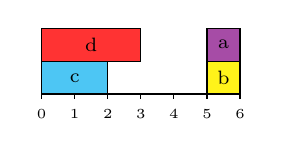
\begin{tikzpicture}[x=0.42cm,y=0.42cm,font=\scriptsize]
\draw[fill=cyan!70] (0,0) rectangle (2,1);\node at (1.0,0.5) {c};
\draw[fill=red!80] (0,1) rectangle (3,2);\node at (1.5,1.5) {d};
\draw[fill=yellow!90] (5,0) rectangle (6,1);\node at (5.5,0.5) {b};
\draw[fill=violet!70] (5,1) rectangle (6,2);\node at (5.5,1.5) {a};
\draw[thick] (0,0) -- (6,0);
\draw (0,0) -- (0,-0.15) node[below,font=\tiny] {0};
\draw (1,0) -- (1,-0.15) node[below,font=\tiny] {1};
\draw (2,0) -- (2,-0.15) node[below,font=\tiny] {2};
\draw (3,0) -- (3,-0.15) node[below,font=\tiny] {3};
\draw (4,0) -- (4,-0.15) node[below,font=\tiny] {4};
\draw (5,0) -- (5,-0.15) node[below,font=\tiny] {5};
\draw (6,0) -- (6,-0.15) node[below,font=\tiny] {6};
\end{tikzpicture}\\[2pt] $S_{2}$\end{minipage}\\[8pt]
\begin{minipage}[b]{0.31\textwidth}\centering
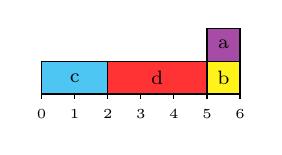
\begin{tikzpicture}[x=0.42cm,y=0.42cm,font=\scriptsize]
\draw[fill=cyan!70] (0,0) rectangle (2,1);\node at (1.0,0.5) {c};
\draw[fill=red!80] (2,0) rectangle (5,1);\node at (3.5,0.5) {d};
\draw[fill=yellow!90] (5,0) rectangle (6,1);\node at (5.5,0.5) {b};
\draw[fill=violet!70] (5,1) rectangle (6,2);\node at (5.5,1.5) {a};
\draw[thick] (0,0) -- (6,0);
\draw (0,0) -- (0,-0.15) node[below,font=\tiny] {0};
\draw (1,0) -- (1,-0.15) node[below,font=\tiny] {1};
\draw (2,0) -- (2,-0.15) node[below,font=\tiny] {2};
\draw (3,0) -- (3,-0.15) node[below,font=\tiny] {3};
\draw (4,0) -- (4,-0.15) node[below,font=\tiny] {4};
\draw (5,0) -- (5,-0.15) node[below,font=\tiny] {5};
\draw (6,0) -- (6,-0.15) node[below,font=\tiny] {6};
\end{tikzpicture}\\[2pt] $S_{3}$\end{minipage}\hfill
\begin{minipage}[b]{0.31\textwidth}\centering
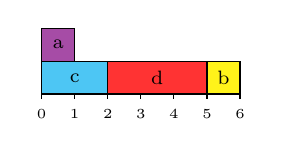
\begin{tikzpicture}[x=0.42cm,y=0.42cm,font=\scriptsize]
\draw[fill=cyan!70] (0,0) rectangle (2,1);\node at (1.0,0.5) {c};
\draw[fill=red!80] (2,0) rectangle (5,1);\node at (3.5,0.5) {d};
\draw[fill=yellow!90] (5,0) rectangle (6,1);\node at (5.5,0.5) {b};
\draw[fill=violet!70] (0,1) rectangle (1,2);\node at (0.5,1.5) {a};
\draw[thick] (0,0) -- (6,0);
\draw (0,0) -- (0,-0.15) node[below,font=\tiny] {0};
\draw (1,0) -- (1,-0.15) node[below,font=\tiny] {1};
\draw (2,0) -- (2,-0.15) node[below,font=\tiny] {2};
\draw (3,0) -- (3,-0.15) node[below,font=\tiny] {3};
\draw (4,0) -- (4,-0.15) node[below,font=\tiny] {4};
\draw (5,0) -- (5,-0.15) node[below,font=\tiny] {5};
\draw (6,0) -- (6,-0.15) node[below,font=\tiny] {6};
\end{tikzpicture}\\[2pt] $S_{4}$\end{minipage}\hfill
\begin{minipage}[b]{0.31\textwidth}\centering
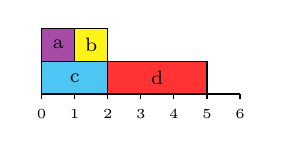
\begin{tikzpicture}[x=0.42cm,y=0.42cm,font=\scriptsize]
\draw[fill=cyan!70] (0,0) rectangle (2,1);\node at (1.0,0.5) {c};
\draw[fill=red!80] (2,0) rectangle (5,1);\node at (3.5,0.5) {d};
\draw[fill=violet!70] (0,1) rectangle (1,2);\node at (0.5,1.5) {a};
\draw[fill=yellow!90] (1,1) rectangle (2,2);\node at (1.5,1.5) {b};
\draw[thick] (0,0) -- (6,0);
\draw (0,0) -- (0,-0.15) node[below,font=\tiny] {0};
\draw (1,0) -- (1,-0.15) node[below,font=\tiny] {1};
\draw (2,0) -- (2,-0.15) node[below,font=\tiny] {2};
\draw (3,0) -- (3,-0.15) node[below,font=\tiny] {3};
\draw (4,0) -- (4,-0.15) node[below,font=\tiny] {4};
\draw (5,0) -- (5,-0.15) node[below,font=\tiny] {5};
\draw (6,0) -- (6,-0.15) node[below,font=\tiny] {6};
\end{tikzpicture}\\[2pt] $S_{5}$\end{minipage}\\[8pt]
\begin{minipage}[b]{0.31\textwidth}\centering
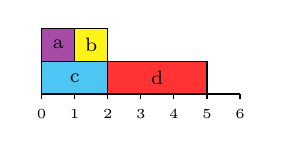
\begin{tikzpicture}[x=0.42cm,y=0.42cm,font=\scriptsize]
\draw[fill=cyan!70] (0,0) rectangle (2,1);\node at (1.0,0.5) {c};
\draw[fill=red!80] (2,0) rectangle (5,1);\node at (3.5,0.5) {d};
\draw[fill=violet!70] (0,1) rectangle (1,2);\node at (0.5,1.5) {a};
\draw[fill=yellow!90] (1,1) rectangle (2,2);\node at (1.5,1.5) {b};
\draw[thick] (0,0) -- (6,0);
\draw (0,0) -- (0,-0.15) node[below,font=\tiny] {0};
\draw (1,0) -- (1,-0.15) node[below,font=\tiny] {1};
\draw (2,0) -- (2,-0.15) node[below,font=\tiny] {2};
\draw (3,0) -- (3,-0.15) node[below,font=\tiny] {3};
\draw (4,0) -- (4,-0.15) node[below,font=\tiny] {4};
\draw (5,0) -- (5,-0.15) node[below,font=\tiny] {5};
\draw (6,0) -- (6,-0.15) node[below,font=\tiny] {6};
\end{tikzpicture}\\[2pt] $S_{6}$\end{minipage}\hfill
\begin{minipage}[b]{0.31\textwidth}\centering
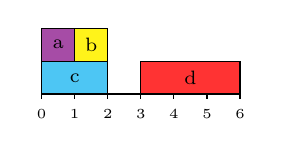
\begin{tikzpicture}[x=0.42cm,y=0.42cm,font=\scriptsize]
\draw[fill=cyan!70] (0,0) rectangle (2,1);\node at (1.0,0.5) {c};
\draw[fill=red!80] (3,0) rectangle (6,1);\node at (4.5,0.5) {d};
\draw[fill=violet!70] (0,1) rectangle (1,2);\node at (0.5,1.5) {a};
\draw[fill=yellow!90] (1,1) rectangle (2,2);\node at (1.5,1.5) {b};
\draw[thick] (0,0) -- (6,0);
\draw (0,0) -- (0,-0.15) node[below,font=\tiny] {0};
\draw (1,0) -- (1,-0.15) node[below,font=\tiny] {1};
\draw (2,0) -- (2,-0.15) node[below,font=\tiny] {2};
\draw (3,0) -- (3,-0.15) node[below,font=\tiny] {3};
\draw (4,0) -- (4,-0.15) node[below,font=\tiny] {4};
\draw (5,0) -- (5,-0.15) node[below,font=\tiny] {5};
\draw (6,0) -- (6,-0.15) node[below,font=\tiny] {6};
\end{tikzpicture}\\[2pt] $S_{7}$\end{minipage}\hfill\caption{Situação 3: $S_0$ a $S_7$ ($S_5$ e $S_6$ coincidem na figura do enunciado).}\end{figure}

\paragraph{Situação 1} ($S_0$: $c@0/0,\ a@3/0,\ b@5/0,\ d@3/1$ --- $d$ em ponte sobre $a$ e $b$).
\begin{center}\footnotesize\begin{tabular}{@{}l@{\ }p{11.2cm}r@{}}\toprule
Meta & Plano manual & Ações\\\midrule
$S_{f3}$ & $\mv(d,c,0)$; $\mv(a,\Tm,2)$ & 2\\
$S_{f4}$ & $\mv(d,c,0)$; $\mv(a,b,5)$; $\mv(d,\Tm,2)$; $\mv(a,c,0)$ & 4\\
$S_{f1}$ & $\mv(d,c,0)$; $\mv(a,\Tm,2)$; $\mv(d,a,1)$; $\mv(b,c,0)$; $\mv(d,\Tm,3)$; $\mv(a,d,4)$; $\mv(b,d,5)$; $\mv(c,a,4)$ & 8\\
$S_{f2}$ & $\mv(c,\Tm,1)$; $\mv(d,c,0)$; $\mv(a,\Tm,0)$; $\mv(d,c,1)$; $\mv(b,a,0)$; $\mv(d,\Tm,3)$; $\mv(c,d,4)$; $\mv(b,c,5)$; $\mv(a,c,4)$ & 9\\\bottomrule
\end{tabular}\end{center}
Execução detalhada de $S_{f4}$:
\begin{center}\small\begin{tabular}{@{}clp{7.6cm}@{}}\toprule
$t$ & Ação & Verificação e novo estado\\\midrule
0 & $\mv(d,c,0)$ & $\clr(d)$; slots 0--2 do nível 1 livres; apoio: slots 0,1 ($c$) $=2\ge2$. $d@0/1$\\
1 & $\mv(a,b,5)$ & $\clr(a)$; slot 5 do nível 1 livre; apoio $b$. $a@5/1$\\
2 & $\mv(d,\Tm,2)$ & slots 2--4 do nível 0 livres (a saiu do slot 3). $d@2/0$\\
3 & $\mv(a,c,0)$ & slot 0 do nível 1 livre; apoio $c$. $a@0/1$ $\Rightarrow$ $S_{f4}$\\\bottomrule
\end{tabular}\end{center}
Observação: o plano de exemplo do esboço do manual (``$a$ para a mesa em $p=4$ e depois $d$ para a mesa em $p=2$'') é inválido, pois $d$ cobriria o slot 4, ocupado por $a$.

\paragraph{Situação 2} ($S_0$: $c@0/0,\ d@3/0,\ a@0/1,\ b@1/1$), meta $S_5$: $d@3/0,\ c@4/1,\ a@4/2,\ b@5/2$.
\begin{center}\small\begin{tabular}{@{}clp{7.6cm}@{}}\toprule
$t$ & Ação & Novo estado / observação\\\midrule
0 & $\mv(a,d,3)$ & $a@3/1$ (apoio: slot 3 de $d$)\\
1 & $\mv(b,a,3)$ & $b@3/2$ (estaciona $b$ sobre $a$)\\
2 & $\mv(c,d,4)$ & $c$ ficou livre; $c@4/1$, slots 4,5 sobre $d$\\
3 & $\mv(b,c,5)$ & $b@5/2$\\
4 & $\mv(a,c,4)$ & $a@4/2$ $\Rightarrow$ $S_5$\\\bottomrule
\end{tabular}\end{center}

\paragraph{Situação 3} ($S_0$ igual ao da Situação 1), meta $S_7$: $c@0/0,\ a@0/1,\ b@1/1,\ d@3/0$.
\begin{center}\small\begin{tabular}{@{}clp{7.6cm}@{}}\toprule
$t$ & Ação & Estado do enunciado atingido\\\midrule
0 & $\mv(d,c,0)$ & $S_1$\\
1 & $\mv(a,b,5)$ & $S_2$\\
2 & $\mv(d,\Tm,2)$ & $S_3$\\
3 & $\mv(a,c,0)$ & $S_4$\\
4 & $\mv(b,c,1)$ & $S_5=S_6$ ($d@2/0$)\\
5 & $\mv(d,\Tm,3)$ & $d$ desliza para $[3,6)$ $\Rightarrow$ $S_7$\\\bottomrule
\end{tabular}\end{center}

%====================================================================
\section{Codificação CNF}
\subsection{Variáveis proposicionais}
Para $t\in\{0,\dots,T\}$ (estado) e $t<T$ (ação). A relação $\mathit{on}$ \emph{não} é codificada; é derivada na interpretação.
\begin{center}\small\begin{tabular}{@{}llp{6.4cm}r@{}}\toprule
Variável & Índices & Significado & Qtd.\ por $t$\\\midrule
$\at(b,p,t)$ & $p\in[0,6-\len(b)]$ & $b$ começa em $p$ & 21\\
$\lev(b,l,t)$ & $l\in[0,3]$ & $b$ está no nível $l$ & 16\\
$\clr(b,t)$ & & topo de $b$ livre & 4\\
$\mathit{cob}(b,s,t)$ & $s\in[0,5]$ & $b$ cobre o slot $s$ (aux.) & 24\\
$\mathit{ocb}(b,s,l,t)$ & & $b$ ocupa a célula $(s,l)$ (aux.) & 96\\
$\mathit{ocp}(s,l,t)$ & & alguém ocupa $(s,l)$ (aux.) & 24\\
$\mv(b,y,p,t)$ & $y\in B\setminus\{b\}\cup\{\Tm\}$ & ação (somente $t<T$) & 84\\\bottomrule
\end{tabular}\end{center}
Total: $|V|=185\,(T+1)+84\,T = 269\,T+185$ (por exemplo, $T=4$: $1261$ variáveis).

\subsection{Grupos de cláusulas}
\begin{enumerate}\setlength\itemsep{2pt}
\item \textbf{Estado inicial} e \textbf{meta}: unitárias $\at(b,p,0),\lev(b,l,0)$ e $\at(b,p,T),\lev(b,l,T)$.
\item \textbf{Unicidade} (A,B): para cada $b,t$: $\bigvee_p\at(b,p,t)$ e $\neg\at(b,p_1,t)\vee\neg\at(b,p_2,t)$; análogo para $\lev$.
\item \textbf{Geometria} (definições): $\mathit{cob}\leftrightarrow\bigvee_{p:\,s\in\mathrm{span}(b,p)}\at(b,p,t)$; $\mathit{ocb}\leftrightarrow\mathit{cob}\wedge\lev$; $\mathit{ocp}\leftrightarrow\bigvee_b\mathit{ocb}$.
\item \textbf{Exclusão horizontal} (C): $\neg\mathit{ocb}(b_1,s,l,t)\vee\neg\mathit{ocb}(b_2,s,l,t)$.
\item \textbf{Estabilidade} (D): para $l>0$: $\neg\at(b,p,t)\vee\neg\lev(b,l,t)\vee\bigvee_{s\in S}\mathit{ocp}(s,l-1,t)$ para todo subconjunto $S$ do span com $|S|=\len(b)-\lceil\len(b)/2\rceil+1$ (``pelo menos $k$ de $n$'' $\equiv$ todo subconjunto de tamanho $n-k+1$ contém um verdadeiro).
\item \textbf{Clear} (E): $\clr(b,t)\leftrightarrow\bigwedge_{s\in\mathrm{span}}\neg\mathit{ocp}(s,l+1,t)$, condicionado a $\at(b,p,t)\wedge\lev(b,l,t)$.
\item \textbf{Ação única} (F): $\neg\mv_1\vee\neg\mv_2$ para todo par em $t$ (permite $\le1$ ação por passo; o menor $T$ com SAT dá o plano mínimo).
\item \textbf{Pré-condições de $\mv(b,y,p,t)$} (G): $\neg m\vee\clr(b,t)$; $\neg m\vee\neg\at(y,p_y,t)$ para $p_y$ sem sobreposição; para cada nível $l_y$ de $y$: slots-alvo livres $\neg m\vee\neg\lev(y,l_y,t)\vee\neg\mathit{ocb}(x,s,l_y+1,t)$ ($x\ne b$); proibição de no-op; $y$ no nível máximo $\Rightarrow\neg m$.
\item \textbf{Efeitos} (H): $\neg m\vee\at(b,p,t+1)$ e $\neg m\vee\neg\lev(y,l_y,t)\vee\lev(b,l_y+1,t+1)$ (ou $\lev(b,0,t+1)$ se $y=\Tm$).
\item \textbf{Frame} (I): $\neg\at(x,p,t)\vee\at(x,p,t+1)\vee\bigvee_{m\ \text{move de }x}m$; análogo para $\lev$. Não há frame para $\clr$ (derivado).
\end{enumerate}

%====================================================================
\section{Exemplos dos 3 cenários codificados para CNF}
\subsection{Situação 1, meta $S_{f4}$, $T=4$}
\begin{lstlisting}
p cnf 1261 26397
13 0     <- at(c,0,0)
 4 0     <- at(a,3,0)
12 0     <- at(b,5,0)
21 0     <- at(d,3,0)
30 0  26 0  22 0  35 0   <- lev(c,0,0) lev(b,0,0) lev(a,0,0) lev(d,1,0)
\end{lstlisting}
A ação $\mv(d,c,0,0)$ é a variável 1002. Algumas de suas cláusulas:
\begin{lstlisting}
-1002 41 0     # move(d,c,0,0) -> clr(d,0)
-1002 203 0    # move(d,c,0,0) -> at(d,0,1)
-1002 -16 0    # move(d,c,0,0) -> not at(c,3,0)   (c nao sobrepoe o span de d)
-1002 -17 0    # move(d,c,0,0) -> not at(c,4,0)
-1002 -30 220 0  # (c no nivel 0) -> lev(d,1,1)
\end{lstlisting}
\subsection{Situações 2 e 3}
Mudam apenas \texttt{INITIAL} e \texttt{GOAL} (arquivo \texttt{src/cenarios.py}):
\begin{center}\small\begin{tabular}{@{}lllrr@{}}\toprule
Cenário & Estado inicial & Meta principal & $T^*$ & Cláusulas\\\midrule
1 & $c@0/0,a@3/0,b@5/0,d@3/1$ & $S_{f4}$ & 4 & 26\,397\\
2 & $c@0/0,d@3/0,a@0/1,b@1/1$ & $S_5$ & 5 & 32\,752\\
3 & mesmo do cenário 1 & $S_7$ & 6 & 39\,107\\\bottomrule
\end{tabular}\end{center}

%====================================================================
\section{Mapeamento: Descrição Formal $\to$ Código}
\begin{center}\small\begin{tabular}{@{}p{5.6cm}p{8.6cm}@{}}\toprule
Regra formal & Código (\texttt{src/bw2cnf\_var.py})\\\midrule
Blocos, comprimentos, pontos & \texttt{BLOCKS, LEN, MAX\_POINT} em \texttt{cenarios.py}\\
Posições válidas $0..6-\len(b)$ & \texttt{positions(b)}\\
Span, sobreposição & \texttt{span(b,p)}, \texttt{spans\_overlap}\\
$\at,\lev,\clr,\mv$ & \texttt{self.novo('at',b,p,t)} etc.\ (\texttt{criar\_variaveis})\\
Estado inicial / meta & \texttt{estado\_inicial}, \texttt{meta\_final}\\
Unicidade (A,B) & \texttt{axiomas\_estado}, \texttt{exatamente\_um}\\
Geometria & \texttt{geometria}\\
Exclusão horizontal (C) & \texttt{exclusao\_horizontal}\\
Estabilidade (D) & \texttt{estabilidade}\\
Clear (E) & \texttt{clear}\\
Ação única (F) & \texttt{axiomas\_acao}\\
Pré/efeitos (G,H) & \texttt{move}, \texttt{efeitos\_nivel}\\
Frame (I) & \texttt{frame}\\
Relação $\mathit{on}$ derivada & \texttt{interpretar.py:derivar\_on}\\
Ordem parcial & \texttt{interpretar.py:ordem\_parcial}\\
Oráculo & \texttt{oraculo\_bfs.py}\\\bottomrule
\end{tabular}\end{center}

%====================================================================
\section{Execução Passo a Passo}
\begin{lstlisting}
pip install python-sat            # so se nao houver o binario minisat
cd src
python3 bw2cnf_var.py --cenario 1 --alvo Sf4 --horizonte 4 --saida ../cenario1
   # Gerado: 1261 variaveis, 26397 clausulas
minisat ../cenario1/trab01_blocos2SAT.cnf ../cenario1/resultado1.txt
python3 interpretar.py ../cenario1/resultado1.txt --mapa ../cenario1/trab01_blocos2SAT.map --verbose --verificar
python3 rodar_sat.py --cenario 1 --alvo Sf4 --saida ../cenario1   # busca T minimo (T=0,1,...)
python3 rodar_todos.py            # todos os cenarios e alvos + resumo
\end{lstlisting}
\texttt{rodar\_sat.py} usa o binário \texttt{minisat} se existir; caso contrário usa o MiniSat 2.2 do PySAT, com o mesmo formato de saída.
Os resultados de todos os alvos estão em \texttt{cenarioN/<alvo>/}; os arquivos do enunciado
(\texttt{trab01\_blocos2SAT.cnf/.map}, \texttt{resultado1/2/3.txt}) estão em \texttt{cenario1/}, \texttt{cenario2/}, \texttt{cenario3/}.

%====================================================================
\section{Interpretação da Saída do SAT Solver}
O miniSAT devolve apenas inteiros (todos os literais, com sinal). Para $S_{f4}$, os literais positivos que são ações são
\texttt{1002, 1015, 1176, 1184}, e o \texttt{.map} os traduz:
\begin{lstlisting}
1002 mv(d,c,0,0)   1015 mv(a,b,5,1)   1176 mv(d,T,2,2)   1184 mv(a,c,0,3)
\end{lstlisting}
\texttt{interpretar.py} (i) lê o mapa; (ii) mantém os literais positivos; (iii) reconstrói $\at,\lev$ por $t$ e as ações; (iv) deriva
$\mathit{on}$ (nível 0 $\Rightarrow$ mesa; senão blocos do nível $l-1$ cujo span sobrepõe o de $b$, vários $\Rightarrow$ ponte); (v) calcula a ordem parcial; (vi) com \texttt{--verificar}
re-executa o plano no oráculo (independente do SAT) e testa as linearizações:
\begin{lstlisting}
PLANO ENCONTRADO (4 acoes):
1. t=0: mover bloco 'd' para CIMA de 'c' em p=0
2. t=1: mover bloco 'a' para CIMA de 'b' em p=5
3. t=2: mover bloco 'd' para a MESA em p=2
4. t=3: mover bloco 'a' para CIMA de 'c' em p=0
ESTADO FINAL (t=4): a esta sobre: c ; b, c, d na MESA
ORDEM PARCIAL: 1<2 [causal: celula(slot 3, nivel 1)]  2<3 [causal: celula(slot 3, nivel 0)]
               3<4 [causal: celula(slot 0, nivel 1)]
VERIFICACAO: plano valido no oraculo = True
\end{lstlisting}
\paragraph{Ordem parcial no cenário $S_5$.} O plano do SAT é $\mv(b,d,3)$; $\mv(a,\Tm,2)$; $\mv(c,d,4)$; $\mv(a,c,4)$; $\mv(b,c,5)$.
As ações 1 e 2 são independentes, e as ações 4 e 5 só dependem de 3:
\begin{center}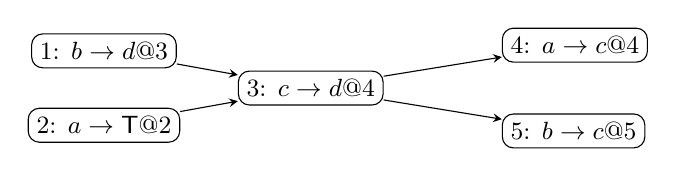
\begin{tikzpicture}[>=stealth,node distance=1.6cm,every node/.style={draw,rounded corners,font=\small,inner sep=3pt}]
\node(a1){1: $b\to d@3$};\node[below=0.5cm of a1](a2){2: $a\to\Tm@2$};
\node[right=1.7cm of $(a1)!0.5!(a2)$](a3){3: $c\to d@4$};
\node[above right=0.1cm and 1.5cm of a3](a4){4: $a\to c@4$};\node[below right=0.1cm and 1.5cm of a3](a5){5: $b\to c@5$};
\draw[->](a1)--(a3);\draw[->](a2)--(a3);\draw[->](a3)--(a4);\draw[->](a3)--(a5);
\end{tikzpicture}\end{center}
Cada ordem topológica (4 no total) foi executada com sucesso no oráculo.

\end{document}
